\documentclass[]{article}

\usepackage{amsmath}
\usepackage{amsfonts}
\usepackage{graphicx,picture,calc}
\usepackage{tikz}
\usepackage{url}
\usepackage{subfig}
\usepackage{listings}
\usepackage{float}

\linespread{2}

\usepackage{lineno}
\linenumbers

\usepackage[affil-it]{authblk}

\lstset{
	basicstyle=\ttfamily,
	columns=fullflexible,
	frame=single,
	breaklines=true,
	postbreak=\mbox{\textcolor{red}{$\hookrightarrow$}\space},
}


\usepackage{natbib}
\bibliographystyle{../mee}
\bibpunct{(}{)}{;}{a}{}{;}

%opening
\title{Web-based supplementary material for Using balanced acceptance sampling as a master sample for environmental surveys}

\author[1,*]{Paul van Dam-Bates}
\author[2]{Oliver Gansell}
\author[3]{Blair Robertson}

\affil[1]{%
	Department of Conservation, Christchurch, New Zealand 
}
\affil[2]{%
	Department of Conservation, Hamilton, New Zealand}

\affil[3]{%
	University of Canterbury, Christchurch, New Zealand}

\affil[*]{Corresponding author: Paul van Dam-Bates, pbates@doc.govt.nz}

\begin{document}
\maketitle

\section{Simulation Study}

 We investigated estimation using the sampling methods balanced acceptance sampling (BAS), generalised random tessellation stratified (GRTS) and altered balanced acceptance sampling (aBAS) for augmenting legacy monitoring. To test differences between the methods, three response surfaces were generated: a strong spatial trend (Population 1), a peak (Population 2), and a cyclical trend (Population 3). The three functions used to define response values are listed below.

\begin{itemize}
	\item
	Population 1 \citep{Robertson2013, Grafstrom2012}:
	\begin{equation*}
	f(\boldsymbol{x}) = 1000\left[3(x_1 + x_2) + \sin(6(x_1 + x_2))\right],
	\end{equation*}
	with population total $\tau \approx 2999.4$ (see Figure \ref{figpop}(a)).
	\item
	Population 2 (Peak function):
	\begin{equation*}
	\begin{split}
	f(\boldsymbol{x}) = 10^6\left[\right.3(4-6x_1)^2 \exp(-(6x_1-3)^2-(6x_2-2)^2) \mathellipsis \\ - 10(0.2(6x_1-3)-(6x_1-3)^3-(6x_2-3)^5)\exp(-(6x_1-3)^2-(6x_2-3)^2) \mathellipsis \\ - \frac{1}{3} \exp(-(6x_1-2)^2-(6x_2-3)^2)\left.\right],
	\end{split}
	\end{equation*}
	with population total $\tau \approx 36270$ (see Figure \ref{figpop}(b)).
	\item
	Population 3 (Bird function):
	\begin{equation*}
	\begin{split}
	f(\boldsymbol{x}) = 1000\left[\right.(12x_1-12x_2)^2 + \exp[(1 - \sin(12x_1-6))^2]\cos(12x_2-6) \mathellipsis \\ + \exp[(1 - \cos(12x_2-6))^2]\sin(12x_1-6)\left.\right],
	\end{split}
	\end{equation*}
	with population total $\tau \approx 23398.2$ (see Figure \ref{figpop}(c)).
\end{itemize}

The sampling frame was defined as $100\times100$ raster in $[0,1)^2$. The response value for each raster cell was defined as the integral of $f(\boldsymbol{x})$ over the cell. Scenarios similar to \citealt{Foster2017} using the program R \citep{R} were run. We assumed an arbitrary overall sample size of $n = 60$. Legacy plots $(n_l \in 3,4,...,57)$ were generated either as simple random samples (SRS) or random-start systematic sampling (SS). More samples $(n_b = 60 - n_l)$ were then included using GRTS \citep{spsurvey}, BAS, and aBAS \citep{MBHdesign}. Simple random samples were added to SS legacy plots as well.

Each raster cell has inclusion probability of $\pi = \frac{n}{100^2}$ when using equal probability sampling. Analysis was carried out for BAS and GRTS as
$$ \bar{y} = \frac{1}{10000} * \sum_{i = 1}^{60} y_i/\pi_i. $$
Where $y_i$ is the observed response value for sample $i$. For aBAS we followed as described in Foster et al. (2017) and calculated the sample mean as
$$ \bar{y} = \frac{1}{10000} * \left( \frac{n_l}{60}\sum_{i = 1}^{n_l} y_i/\pi_l  + \frac{n + n_l}{60}\sum_{i = 1}^{n} y_i/\pi_{ai} \right).$$

For each sample size of $3 \leq n_l \leq 57$ we ran $1000$ simulations.

\newpage

\begin{figure}[H]
	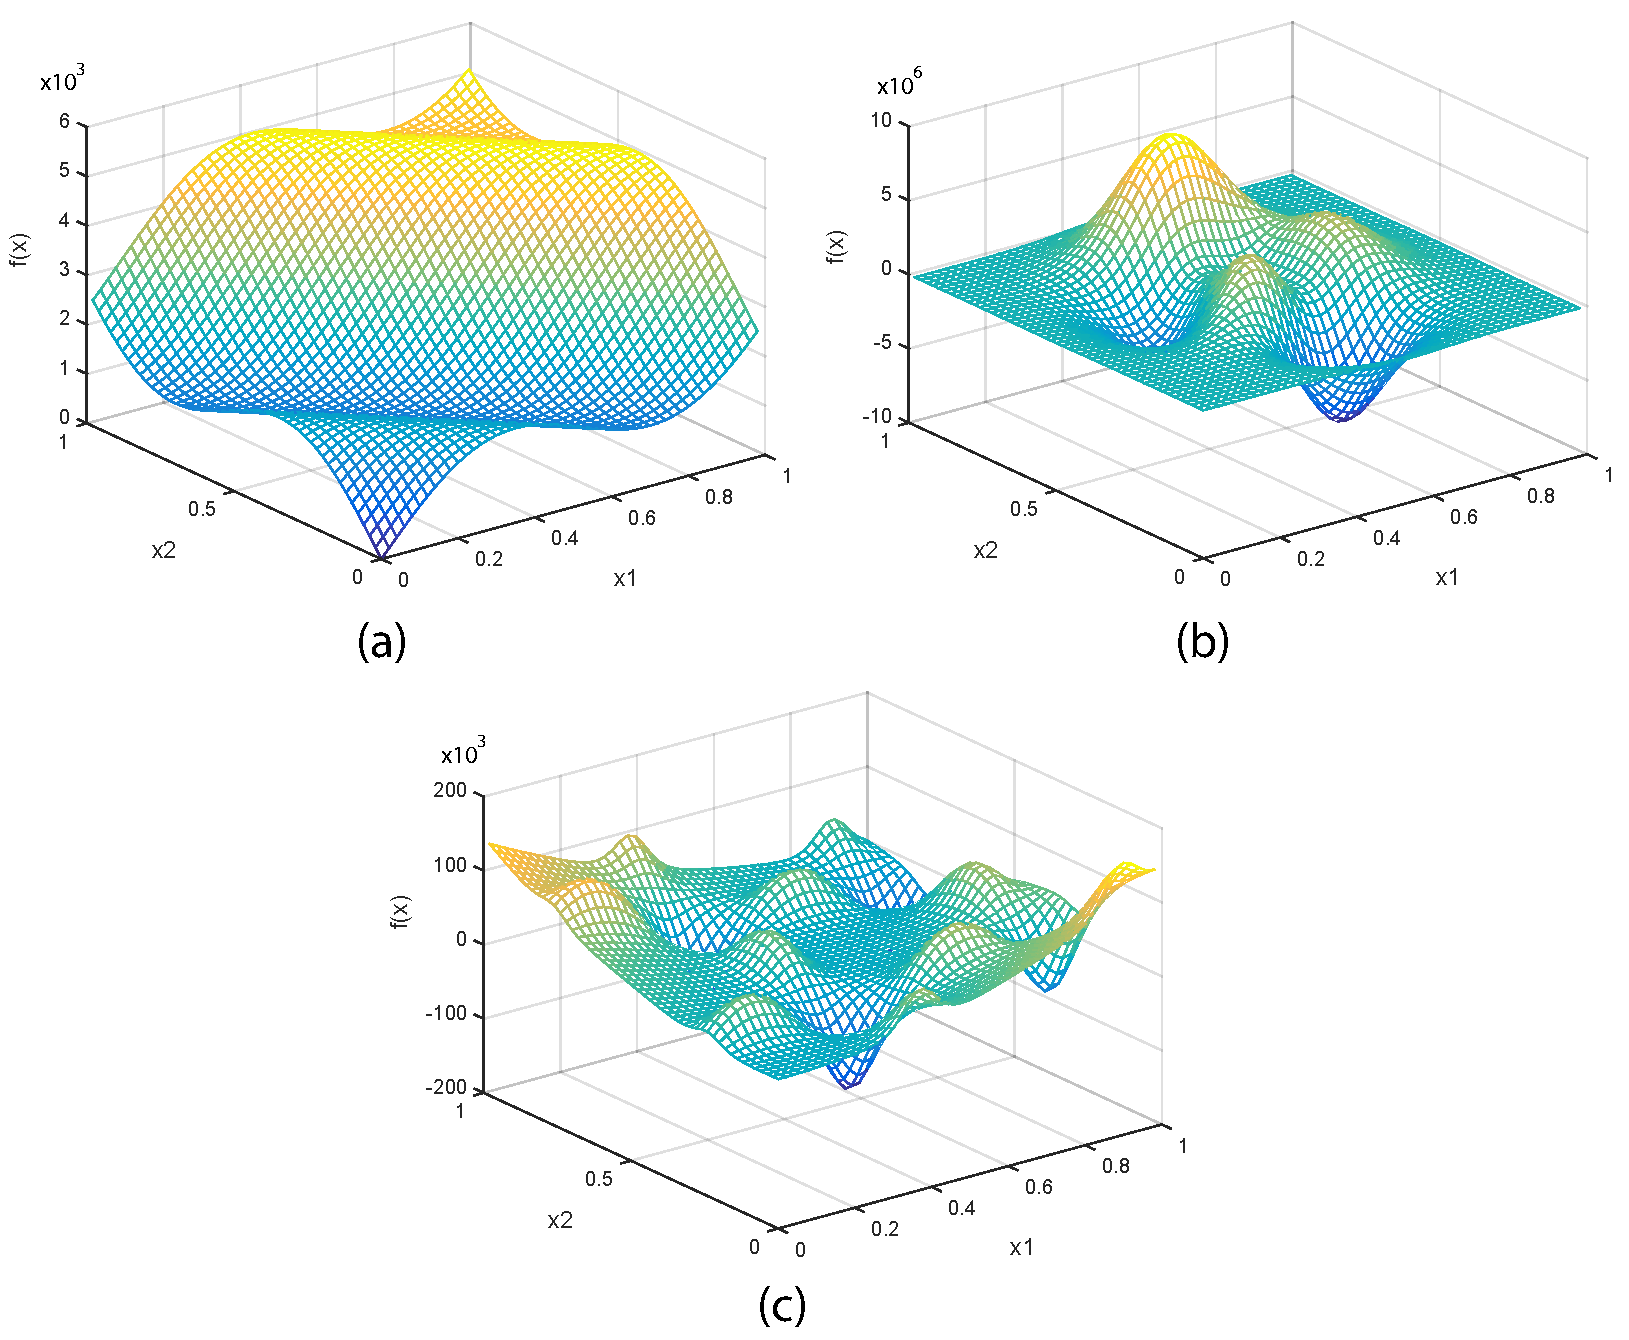
\includegraphics[width = \textwidth]{pop123.eps}
	\caption{The three populations used to test estimation in Section 2.6. (a) Population 1, (b) Population 2 and (c) Population 3.}
	\label{figpop}
\end{figure}

\newpage

\section{Master Sample R Code (NZ)}

\begin{lstlisting}[language=R]
library(sp)

#Halton Sequence:
RSHalton <- function(n = 10,seeds = c(0,0),bases = c(2,3)) {
	##
	## Generate n points from a random start d dimensional Halton sequence.
	##
	## Inputs:
	## 
	## n 			sample size
	## bases    	coprime bases e.g. c(2,3) (Halton Sequence)
	## seeds  		random seeds  e.g. c(0,0) (Halton Sequence)
	
	
	########### Initialize #########################################
	d <- length(bases);	pts <- mat.or.vec(n, d)
	if (length(seeds) != d){
		seeds <- rep(seeds[1],d)
	}
	
	########### Main Loop #########################################
	for (i in 1:d) {
		b <- bases[i];   	u <- seeds[i];	k <- u:(u+n-1);
		xk <- (k %% b)/b;
		for (j in 1:(ceiling(logb(u+n,b)) + 2)) {
			xk <- xk + (floor(k/(b^j)) %% b)/(b^(j+1));
		}
		pts[,i] <- cbind(xk)
	}
	pts <- cbind(1:nrow(pts), pts)
	return(pts)
}

#Generate the master sample after the seeds have been manually set.
masterSample <- function(island = "South", shp, N = 100){
#Master Sample seed for South Island, chosen as first random start that fell into SI
#seed.si <-  c(4887260, 18041662)
#seed.ni <- c(5137598, 8906854)

#Define CRS
nztm <-"+proj=tmerc +lat_0=0 +lon_0=173 +k=0.9996 +x_0=1600000 +y_0=10000000 +ellps=GRS80 +towgs84=0,0,0,0,0,0,0 +units=m +no_defs"

if(island == "South")
{
bb <- data.frame(min = c(1089354,4747979), max = c(1721164,5516919), row.names = c("x","y"))
seed <-  c(4887260, 18041662)
}else if(island == "North")
{
bb <- data.frame(min = c(1510593,5390569), max = c(2092000,6223164), row.names = c("x","y"))
seed <- c(5137598, 8906854)
}else{
cat("ERROR: Define Island for MS \n")
return()
}

#Scale and shift Halton to fit into bounding box
scale.bas <- bb[,2] - bb[,1]
shift.bas <- bb[,1]

draw <- 10000

getSample <- function(k = 0){
if(k == 0){ seedshift <- seed 
}else seedshift <- k*draw + seed
pts <- RSHalton(n = draw, seeds = seedshift, bases = c(2,3))
pts[,2] <- pts[,2]*scale.bas[1] + shift.bas[1]
pts[,3] <- pts[,3]*scale.bas[2] + shift.bas[2]

#Give points a projection, clip them as needed.
tmp.order <- (k*draw + 1):((k+1)*draw)
pts.coord <- SpatialPointsDataFrame(cbind(pts[,2],pts[,3]),proj4string=CRS("+proj=tmerc +lat_0=0 +lon_0=173 +k=0.9996 +x_0=1600000 +y_0=10000000 +ellps=GRS80 +units=m +no_defs"), data.frame(SiteOrder = tmp.order))
return(pts.coord)
}

pts.sample <- getSample()
pts.sample <- pts.sample[shp, ]


if(nrow(pts.sample) < N){
di <- 1
while(nrow(pts.sample) < N){
new.pts <- getSample(k = di)
new.pts <- new.pts[shp, ]
pts.sample <- rbind(pts.sample, new.pts)
di <- di + 1
}
return(pts.sample[1:N,])
} else{
return(pts.sample[1:N,])
}
}



\end{lstlisting}


\bibliography{../MasterSampleLit}	



\end{document}